\section{Experimentaci\'on}

Como fue previamente mencionado, la idea ser\'a estudiar qu\'e par\'ametros optimizan el c\'alculo de RTO. Para realizar esto, dividiremos la experimentaci\'on en dos etapas.

Durante la primera etapa, analizaremos c\'omo evoluciona la estimaci\'on de RTO en el cliente con distintas combinaciones de $\alpha$ y $\mathcal{B}$ para un delay fijo y probabilidad de p\'erdida de paquetes nula. A partir de esta experimentaci\'on nos quedaremos con 4 combinaciones de $\alpha$ y $\mathcal{B}$ que a nuestro crtierio son los mejores para estimar el RTO.

Durante la segunda etapa, observaremos c\'omo se comportan las combinaciones anteriores. Para ello volveremos a analizar como evoluciona la estimaci\'on de RTO en el cliente pero, esta vez, iremos variando el delay y la probabilidad de p\'erdida de paquetes. 

\subsection{Etapa Inicial: Estimacion de $\alpha$ y $\beta$}
Con una probabilidad de error nula y un delay de 0.25 segundos, fijaremos los parametros \'optimos de la estimacion del RTO para los siguientes valores $\alpha$ y $\beta$: 0.25, 0.5, 0.75 y 0.9. La idea es combinar todos con todos, es decir, testear los casos para $\alpha$=0.25 y $\beta$=0.25, $\alpha$=0.25 y $\beta$=0.5 y as\'i sucesivamente hasta llegar a $\alpha$=0.9, $\beta$=0.9.\\

En funci\'on de las distintas combinaciones de $\alpha$ y $\beta$ graficamos la efectividad en la aproximaci\'on del RTO y RTT real, la cantidad de retransmisiones y el RTO obtenido.\\

Antes de mostrar los gr\'aficos obtenidos, algunas aclaraciones sobre los mismos:
\begin{itemize}
	\item Para medir la efectividad en la aproximaci\'on del RTO y el RTT real sacamos un promedio de RTO y RTT para cada experimento, es decir, para cada corrida con un $\alpha$ y $\beta$ determinados, obtuvimos un promedio de RTO y RTT durante la transferencia de los datos. Con estos valores calculados obtuvimos la diferencia entre el RTO promedio y el RTT real y normalizamos los valores. Por otro lado, graficamos los valores normalizados haciendo 1-valor. Esto \'ultimo permite una mejor visualizaci\'on de los resultados en los gr\'aficos ya que si la altura de la barra graficada es m\'as 'alta' quiere decir que el RTO promedio calculado se aproxima m\'as al RTT real. 
	% Explicar en que estan medidos los RTO
	\item Las barras de los gr\'aficos poseen heatmap. Esto es, los colores de las barras varian segu\'n la magnitud Z del gr\'afico.
\end{itemize}

%Explicar heatmap de los graficos (colores de las barras varian segun magnitud Z del grafico)

\subsubsection{Efectividad en la aproximaci\'on del RTO y el RTT Real}
%	explicar normalizacion de valores y 1-valor
%	...graficos 3d de las barras con los alfa y beta variados

\begin{figure}[H]
  \centering	
	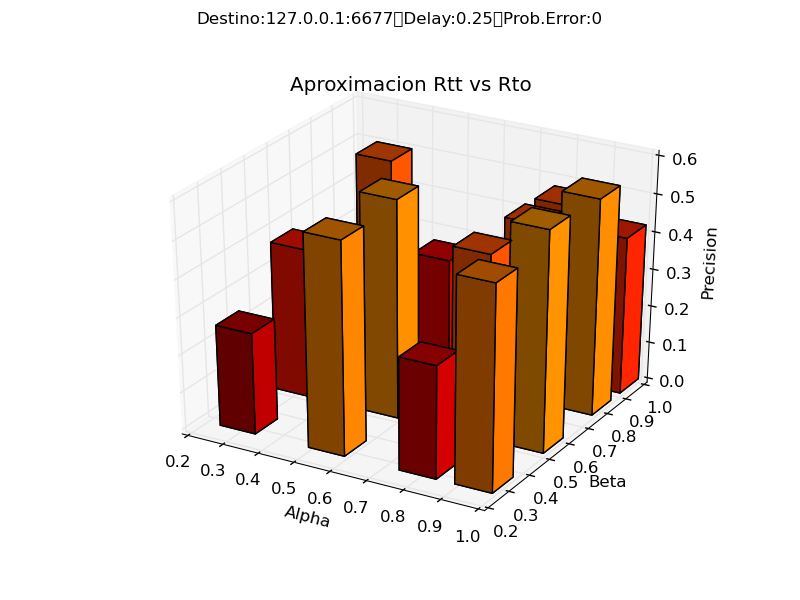
\includegraphics[scale=0.5]{../analisis/graficos_tablas/graficos_en_funcion_de_alfa_y_beta/graficos/rtt_vs_rto.png}
  \caption{Efectividad en la aproximaci\'on del RTO y el RTT Real en funci\'on de $\alpha$ y $\beta$}
	\label{fig:histo-src-sitiotrabajo}
\end{figure}

Observando la figura 1 podemos mencionar que ninguna de las combinaciones de $\alpha$ y $\beta$ super\'o una precisi\'on de 0.6. Sin embargo, observando la altura de las barras, podemos destacar algunas combinaciones que tuvieron resultados por encima de las dem\'as. Estas son:
\begin{itemize}
	\item $\alpha$: 0.5, $\beta$: 0.25
	\item $\alpha$: 0.5, $\beta$: 0.5
	\item $\alpha$: 0.9, $\beta$: 0.5
	\item $\alpha$: 0.9, $\beta$: 0.9
\end{itemize} 

\subsubsection{RTO Estimado}
%	...graficos 3d de las barras con los alfa y beta variados

\begin{figure}[H]
  \centering	
	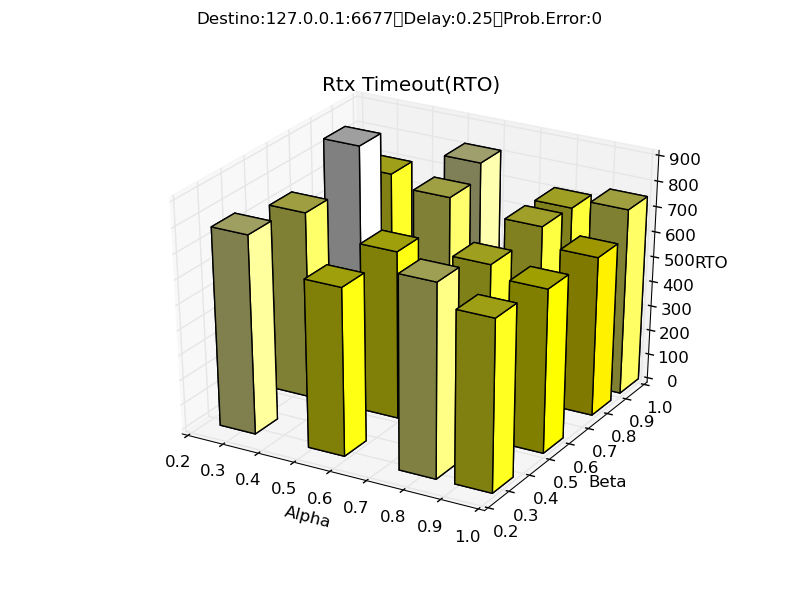
\includegraphics[scale=0.5]{../analisis/graficos_tablas/graficos_en_funcion_de_alfa_y_beta/graficos/rto.png}
  \caption{RTO en funci\'on de $\alpha$ y $\beta$}
	\label{fig:histo-src-sitiotrabajo}
\end{figure}

Este gr\'afico puede complementarse con la figura 1. Mientras m\'as bajos sean los valores de RTO para un $\alpha$ y $\beta$ dados, m\'as cercano estar\'a del RTT real. Esto sucede ya que valores de RTO por debajo del RTT real no tendrian sentido. Si reenviamos un paquete antes del tiempo estimado en que recibimos un ACK, el protocolo retransmitir\'ia siempre, relentizando la comunicaci\'on.

Analizando los resultados obtenidos para cada una de las combinaciones destacadas de la secci\'on 3.1.1 podemos mencionar que los RTO estimados se corresponden con los resultados de antes. Las barras, como podemos observar para estas combinaciones, son las que menos altura tienen respecto de las dem\'as, es decir, el RTO es m\'as bajo y por lo tanto m\'as se aproxima al RTT real.

\subsubsection{Cantidad de retransmisiones}
%	...graficos 3d de las barras con los alfa y beta variados
%	no se que decir de esto

\begin{figure}[H]
  \centering	
	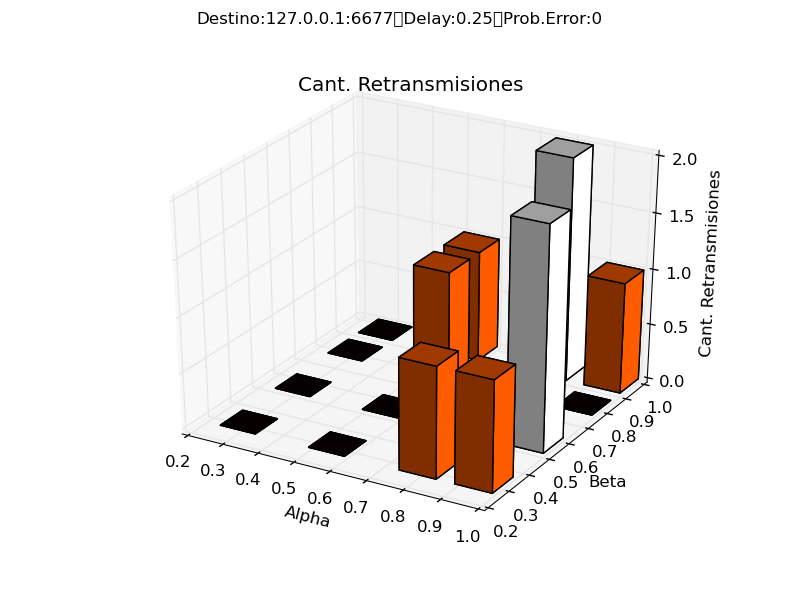
\includegraphics[scale=0.5]{../analisis/graficos_tablas/graficos_en_funcion_de_alfa_y_beta/graficos/retransmisiones.png}
  \caption{Retransmisiones en funci\'on de $\alpha$ y $\beta$}
	\label{fig:histo-src-sitiotrabajo}
\end{figure}

\subsection{Segunda Etapa - Simulacion de problemas de red: Delay y Errores inducidos con probabilidad}